\documentclass[a4paper, 12pt]{article}

%% подключаем стандарт библиографии
\bibliographystyle{gost71u} 

%% for envirovemt "abstract" in class book
%%\newenvironment{abstract}{}{}
\usepackage{abstract}

%% подключаем преамбулу, в ней содержатся подключение всех необходимых пакетов
%%% Работа с русским языком
\usepackage{cmap}			 % поиск в PDF
\usepackage{mathtext} 		 % русские буквы в формулах
\usepackage[T2A]{fontenc}	 % кодировка
\usepackage[utf8]{inputenc}	 % кодировка исходного текста
\usepackage[russian]{babel}	 % локализация и переносы

%%% Пакеты для работы с математикой
\usepackage{amsmath,amsfonts,amssymb,amsthm,mathtools}
\usepackage{icomma}

%% Номера формул
%\mathtoolsset{showonlyrefs=true} % Показывать номера только у тех формул, на которые есть \eqref{} в тексте.
%\usepackage{leqno}               % Немуреация формул слева

%% Шрифты
\usepackage{euscript}	 % Шрифт Евклид
\usepackage{mathrsfs}    % Красивый матшрифт
\usepackage[14pt]{extsizes} % Задаем 14 шрифт

%% Поля (геометрия страницы)
\usepackage[left=3cm,right=2cm,top=2cm,bottom=2cm,bindingoffset=0cm]{geometry}

%% Русские списки
\usepackage{enumitem}
\makeatletter
\AddEnumerateCounter{\asbuk}{\russian@alph}{щ}
\makeatother

%%% Работа с картинками
\usepackage{caption}
\usepackage{subcaption}
\captionsetup{justification=centering} % центрирование подписей к картинкам
\usepackage{graphicx}                  % Для вставки рисунков
\graphicspath{{images/}{images2/}}     % папки с картинками
\setlength\fboxsep{3pt}                % Отступ рамки \fbox{} от рисунка
\setlength\fboxrule{1pt}               % Толщина линий рамки \fbox{}
\usepackage{wrapfig}                   % Обтекание рисунков и таблиц текстом

%%% Работа с таблицами
\usepackage{array,tabularx,tabulary,booktabs} % Дополнительная работа с таблицами
\usepackage{longtable}                        % Длинные таблицы
\usepackage{multirow}                         % Слияние строк в таблице
\usepackage{diagbox}

%% Красная строка
\setlength{\parindent}{2em}

%% Интервалы
\linespread{1.5}
\usepackage{multirow}

%% TikZ
\usepackage{tikz}
\usetikzlibrary{graphs,graphs.standard}

%% Верхний колонтитул
\usepackage{fancyhdr}
\pagestyle{fancy}
\fancyhead[L]{}

%% Перенос знаков в формулах (по Львовскому)
\newcommand*{\hm}[1]{#1\nobreak\discretionary{}{\hbox{$\mathsurround=0pt #1$}}{}}

%% дополнения
\usepackage{float}   % Добавляет возможность работы с командой [H] которая улучшает расположение на странице
\usepackage{gensymb} % Красивые градусы
\usepackage{caption} % Пакет для подписей к рисункам, в частности, для работы caption*

% подключаем hyperref (для ссылок внутри  pdf)
\usepackage[unicode, pdftex]{hyperref}

\begin{document}
    %% титульник
    %%\begin{center}
    %% *название института*
    \textbf{Министерство образования и науки Российской Федерации \\
    Московский физико-технический институт (национальный исследовательский университет)} \\
    \vspace{1cm}

    %% *факультет/физтех-школа*
    Физтех-школа радиотехники и компьютерных технологий \\

    %% *название базовой кафедры и лаборатории*
    %% в случае ненадобности можно удалить
    Кафедра интеллектуальных информационных систем и технологий \\

    \vspace{2em}

    \large{Выпускная квалификационная работа магистра}
\end{center}

\begin{center}
    \vspace{2em}
    %% *название вашей работы*
    \Large{Исследование методов доменной адаптации для улучшения распознавания ключевых точек на теле человека}

    \vspace{\fill}
\end{center}


\begin{flushright}
    \textbf{Автор:} \\
    Студент М01-205а группы \\
    Токарев Андрей Сергеевич \\
    \vspace{2em}
    \textbf{Научный руководитель:} \\
    Доктор технических наук \\
    Назаров Алексей Николаевич \\
    \textbf{Научный конультант:} \\
    Ст. Преподаватель \\
    Воронков Илья Михайлович \\
\end{flushright}

\vspace{1em}

\begin{center}
    %% *лого*
    
\includegraphics[width=100 pt]{MIPT_logo.jpg}\\
    Москва \the\year{}
\end{center}

% выключаем отображение номера для этой страницы (титульник)
\thispagestyle{empty}

\newpage
\setcounter{page}{2}
\fancyfoot[c]{\thepage}
%% *надпись над верхним колонтинулом*
%% в случае ненадобности можно удалить
\fancyhead[L]{Исследование методов доменной адаптации для улучшения распознавания ключевых точек на теле человека}
\fancyhead[R]{}
    %% аннотоция
    \begin{abstract}

    \begin{center}
        \large{Исследование методов доменной адаптации для улучшения распознавания ключевых точек на теле человека} \\
    \large\textit{Токарев Андрей Сергеевич} \\[1 cm]

    %Краткое описание задачи и основных результатов, мотивирующее прочитать весь текст

    \end{center}
    
    \begin{large}
    После достижения хороших результатов в решении задачи распознавания ключевых точек на теле человека и оценки его позы, возникла необходимость уменьшения затрат на улучшение результатов модели на целевых данных. Для решения этой проблемы исследователями были предложены некоторые методы доменной адаптации без учителя, которые позволили значительно ускорить процесс разработки готового решения для узконаправленных задач.
    \end{large}

	\begin{large}
	В рамках данной работы будет представлен анализ как различных моделей оценки позы по ключевым точкам, так и методы доменной адаптации моделей к целевым данным. Также будет представлен анализ работы одного из методов адаптации, хорошо показавшего себя в задачах детекции объектов и повторной идентификации человека.
    \end{large}
    


\end{abstract}
\newpage
    %содержание
    \tableofcontents{}
    \newpage

    \section{Введение}
\label{sec:Chapter0} \index{Chapter0}

Здесь необходимо описать описание проблемы. Ее актуальность. Где это можно использовать и что делать. Заворожить читателя для прочтения твоей работы.
ОПИСАТЬ научную НОВИЗНУ работы.

Современные технологии машинного обучения и компьютерного зрения продолжают активно развиваться, находя применение в самых разнообразных областях. Одно из направлений, активно развивающихся в последние годы, является решение задачи распознавания ключевых точек на теле человека (Keypoint Detection) или оценка позы человека (Human Pose Estimation). На сегодняшний день решения данной задачи могут иметь множество практический применений.(, включая системы наблюдения, анимацию, медицинскую диагностику и интерактивные интерфейсы.)

Одной из возможностей использовать распознавание позы человека является виртуальная реальность. Оцифровка позы человека с помощью неросетей позволяет сэкономить на закупке дорогостоящий костюмов. Можно установить несколько камер, которые будут восстанавливать позу человека и переносить ее компьютерное пространство. При добавлении генеративных алгоритмов можно создавать всевозможные аватары и погрузиться в "Оазис" из фильма Стивена Спилберга "Первому игроку приготовиться".

Другим уже реальным применением данной технологии является рефери спортивных соревнований. Уже сейчас система полуавтоматического определения оффсайда помогает судьям футбольных матчей по всему миру. А работает она на распознавании ключевых точек часте тела, которыми футболист может сыграть в мяч и определяет были ли нарушены правила или гол был забит чисто.  (ССЫЛКА)

Недалеко отходя от спорта, можно применять оценку позы для создания личных тренеров прямо в телефоне. Проект MediaPipe (ССЫЛКА) предлагает уже сейчас возможности для использование его моделей на смартфонах для подсчета количества выполнений таких упражнений, как отжимания, приседания или подтягивания, а также дает возможность оценивать правильность различных асан в йоге.

ЕЩЕ ПРИМЕРОВ ПРО ИСПОЛЬЗОВАНИЕ ЗАДАЧИ ОЦЕНКИ ПОЗЫ

\hfill \break
Обучение модели и разработка алгоритма её работы представляют собой чрезвычайно сложный и трудоемкий процесс. Этот процесс требует значительных ресурсов, как со стороны специалистов, так и в плане вычислительной мощности. Сначала необходимо собрать и подготовить данные, затем обучить модель, настроить её параметры и протестировать на различных наборах данных, чтобы убедиться в её точности и надёжности. Это часто занимает много времени и требует значительных финансовых вложений. 

Данные, на которых модели обучаются имеют общий характер и могут не подходить под определенную узко-специализированную задачу. Например, в футболе не особо важны ключевые точки рук и лица, но важны ключевые точки тела, ног и общая точка головы. Для адаптации модели под данную задачу необходимо проделать гигантсикй объем работы по сбору данных, их фильтрации и разметке. Особенно выделяется последняя часть работы, так как она требует работы нескольких экспертов, которые расставят точки на каждой отобранной фотографии или кадре видео.

Для избежания дополнительных работ по адаптации широкоспециализированной модели к узкой задаче ученые задумались над вопросом приспосабливания модели к новым запросам. Таким образом появилась такая область науки о нейросетях, как адаптация модели к новым доменам данных (англ. Domain Adaptation). ЧТО ТАКОЕ ДОМЕНЫ. КАК МОЖНО АДАПТИРОВАТЬ. ЧТО МОЖНО ИЗ ЭТОГО ПОЛУЧАТЬ.

ДУМАЮ ТУТ ЕЩЁ СТОИТ СКАЗАТЬ ПРО ПЕРЕНОС ОБУЧЕНИЯ.

\hfill \break
В конце стоит описать план по главам и что там будет описано. Кратко и по делу.

В данной работе будет рассмотрено применение алгоритма доменной адаптации Progressive Unsupervised Learning для нескольких решений задачи распознавания ключевых точек на теле человека. Также будут представлены качественные и количественные результаты проведенного эксперимента.


\newpage %% Введение
    \section{Сверточные нейронные сети}
\label{sec:Chapter1} \index{Chapter1}

На анный момент раздел находится под вопросом. Надо узнать насколько необходимо о СНС описывать тут. Если не будет хватать объема, то точно придется дополнять.

\newpage %% Сверточные нейронные сети
    \section{Распознавание ключевых точек}
\label{sec:Chapter2} \index{Chapter2}

С развитием технологий человечество начало ставить все более разнообразные задачи, для решения которых применялись сверточные нейронные сети (convolutional neural network, CNN). Одной из таких задач оказалось распознавание ключевых точек (Keypoint Detection). При этом распознавание ключевых точек на теле человека выделилось в отдельный раздел, известный как оценка позы (Pose Estimation). Далее рассмотрим формулировку этих задач.

\subsection{Ключевые точки}

Задача распознавания ключевых точек заключается в том, чтобы обнаружить и точно локализовать определенные точки или места внутри изображения или кадра видео. Эти точки, называемые ключевыми, могут быть определены для различных объектов, таких как лица, тела человека или других структур. Например, в случае распознавания лица ключевые точки могут включать углы глаз, кончик носа, уголки рта и другие характерные особенности лица. В контексте человеческого тела ключевыми точками могут быть суставы, такие как локти, колени, плечи и так далее. Для других объектов ими могут быть выбраны уникальные элементы, которые помогают идентифицировать и анализировать заданный предмет.

Другими словами, ключевые точки являются структурными, которые используются для определения положения и/или местонахождения объекта в пространстве. Они играют важную роль в задачах компьютерного зрения, таких как отслеживание движений, 3D-моделирование, анимация, медицинская визуализация и другие. Они могут использоваться для создания каркасов объектов, анализа их формы, измерения расстояний между различными частями и выполнения других аналитических задач.

Более точно эти объекты можно определить следующим образом: \textit{ключевые точки (КТ)} - это специфические, заранее определенные части распознаваемого объекта, которые имеют особое значение для дальнейшего анализа местоположения объекта на изображении. Каждая ключевая точка обычно соответствует определенной анатомической или структурной особенности, которая легко распознается и может служить ориентиром для алгоритмов обработки изображений. Иными словами, КТ необходимо обладать следующими характеристиками, чтобы можно было использовать их в качестве референсных для заданного объекта:
\begin{enumerate}
\item \textit{Уникальность}\\
Точки должны быть уникальными и отличаться от других точек на изображении
\item \textit{Инвариантность} \\
Точки должны сохранять свою идентичность при общих преобразованиях изображения, таких как вращение, масштабирование и изменения условий освещения 
\item \textit{Повторяемость} \\
Точки должны быть обнаруживаемы в разных экземплярах одного и того же объекта или сцены
\end{enumerate}

Для анализа структуры объекта и взаимосвязи между его различными КТ часто применяется схематичное описание, которое обеспечивает более наглядное визуальное представление. Этот метод помогает лучше понять анатомическую и функциональную структуру распознаваемого предмета. При этом саму схему, представляющую собой своего рода <<скелет>>, принято называть \textit{топологией}. Примеры различных топологий представлены на \autoref{fig:topology_exaples}.

\begin{figure}[h]
\begin{subfigure}[b]{0.48\textwidth}
	\centering
	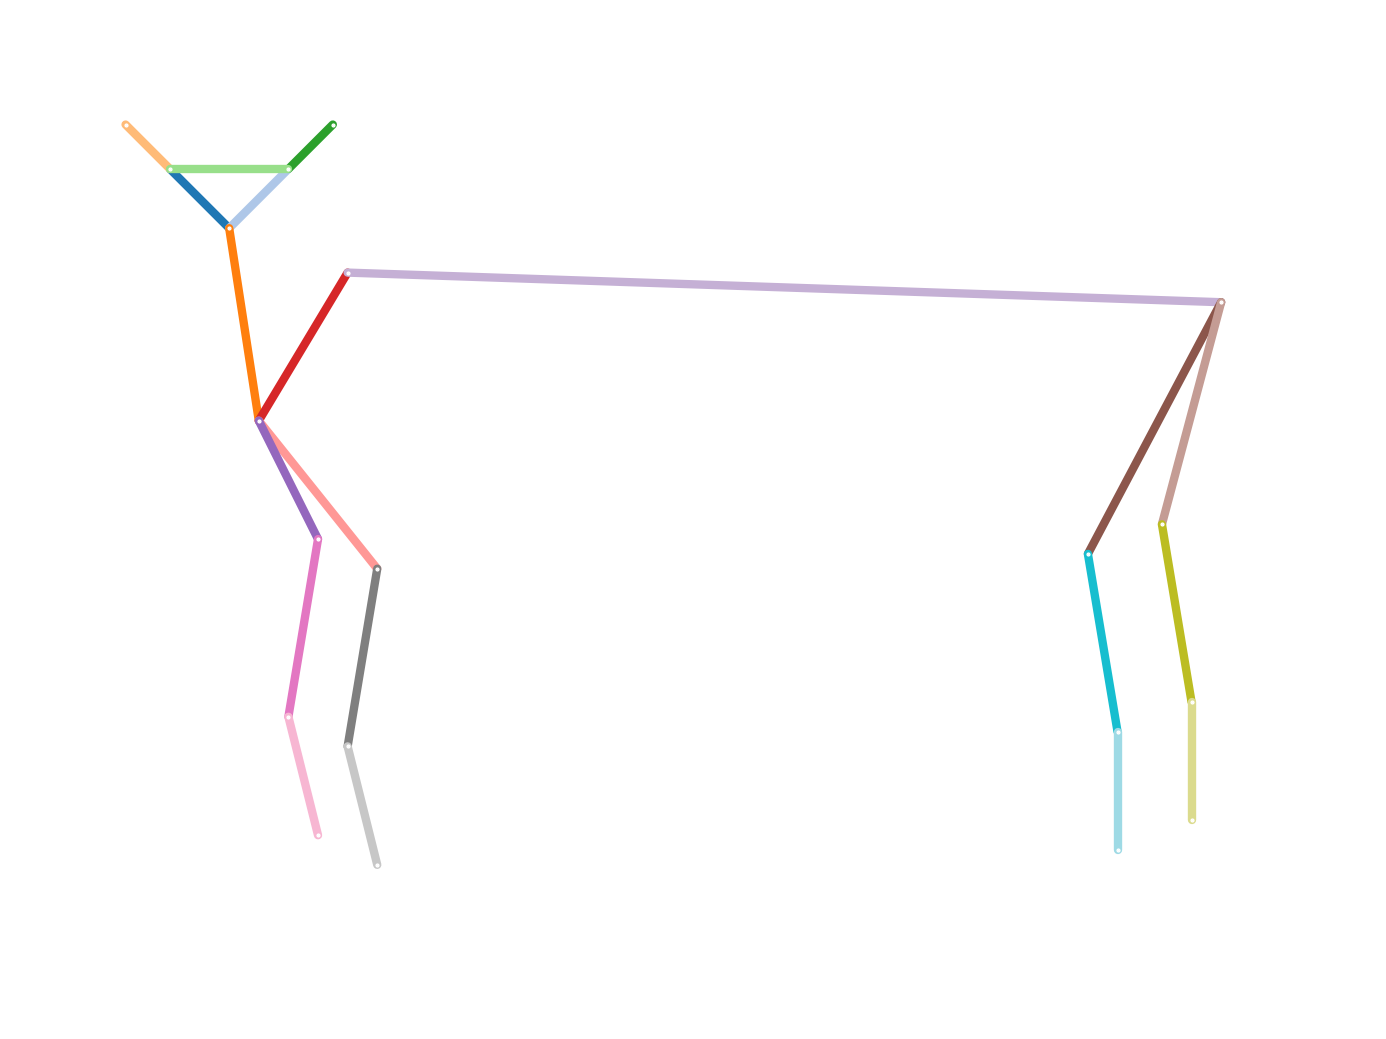
\includegraphics[width=\textwidth]{./images/plugins_animalpose.png}
	\caption{Animal keypoints}
\end{subfigure}
\begin{subfigure}[b]{0.48\textwidth}
	\centering
	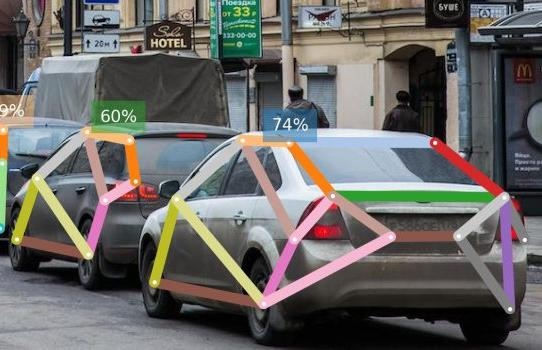
\includegraphics[width=\textwidth]{./images/car_topology.jpg}
	\caption{Car keypoints}
\end{subfigure}
	\caption{Примеры топологий объектов от OpenPifPaf \cite{OpenPifPaf2021}}
	\label{fig:topology_exaples}
\end{figure}

\subsection{Формальная постановка задачи}
\label{subsec:keypoint_task}

Пусть дано изображение $I \in \mathbb R^{H \times W \times C},$ где $H \times W$ - размеры изображения, а $C$ - количество каналов, равное 3 для RGB изображений.

Пусть также задан набор ключевых точек для данного изображения $K \in \mathbb R^{N_c \times N_k}$, где $N_c$ - размерность предсказанных результатов, которая часто равняется размерности выходного пространства с добавлением координаты видимости точки, а $N_K$ - количество ключевых точек.

Тогда задача $T$, выполняющая распознавание ключевых точек определяется как:
$$T = \{K, F_{\theta}(I)\},$$

где $F_{\theta}: \mathbb R^{H \times W \times C} \to \mathbb R^{N_c \times N_k}$ - функция предсказания нейросети с параметрами $\theta$.

Для оценки предсказания $\hat{K} = F_{\theta}(I)$ вводится функция потерь, которую называют KeypointMSELoss: $$L(\hat{K}, K) = \sum_{i=1}^{N_k} ||\hat{K_i} - K_i||^2$$ 

\hfill \break

Процесс обучения нейросети заключается параметров $\theta$ путем минимизации описанной функции потерь на тренировочном наборе размера $N$: $$\theta = argmin_{\theta} \frac{1}{N} \sum_{i=1}^{N} L(F_{\theta}(I_i), K_i)$$

Итоговая формулировка звучит следующим образом:\\
Необходимо найти такую функцию предсказания $F_{\theta}: \mathbb R^{H \times W \times C} \to \mathbb R^{N_c \times N_k}$, которая для входного изображения $I$ и набора реальных ключевых точек $K$ предсказывает ключевые точки $\hat{K}$, минимизируя ошибку по заданной функции потерь $L(\hat{K}, K)$. 


\subsection{Распознавание позы человека}

На теле человека тоже можно выделить несколько ключевых точек, информация о которых дает возможность цифровизовать позу человека и использовать ее для аналитики с помощью методов машинного обучения. Именно для этого и была разработана задача распознавания ключевых точек на теле человека  или, как ее часто называют в англоязычной литературе, задача оценки позы человека (Human Pose Estimation).

\subsubsection*{Расположение ключевых точек. Топология}

Основной вопросом для HPE стал выбор набора ключевых точек и топологии, по которой они будут соединяться.

\begin{figure}[h]
\centering
\begin{subfigure}[b]{.16\textwidth}
	\centering
	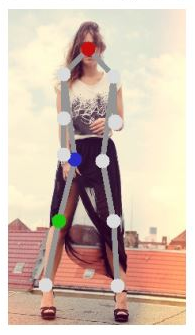
\includegraphics[width=\textwidth]{./images/regpose_topology.png}
	\caption{PDJR \cite{PDJR}}
\end{subfigure}
\begin{subfigure}[b]{.3\textwidth}
	\centering
	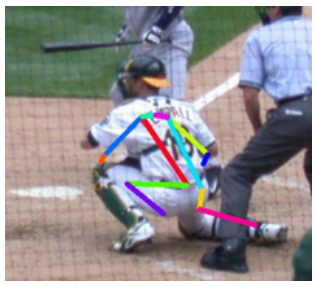
\includegraphics[width=\textwidth]{./images/deeppose_topology.png}
	\caption{DeepPose \cite{DeepPose}}
\end{subfigure}
\begin{subfigure}[b]{.455\textwidth}
	\centering
	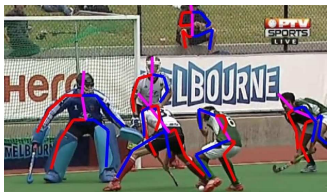
\includegraphics[width=\textwidth]{./images/alphapose_topology.png}
	\caption{AlphaPose \cite{AlphaPose}}
\end{subfigure}
\caption{Примеры различных топологий у первых решений задачи распознавания ключевых точек на теле человека}
\label{fig:topology_examples}
\end{figure}

В первых работах были представлены различные примеры топологий, некоторые примеры представлены на \autoref{fig:topology_examples}. Если точки туловища имеют большое количество пересечений, то точки головы сильно отличались: где-то учитывалось только положение головы (то есть добавлена верхняя точка головы), где-то рассматривались некоторые точки на лице, где-то голова вообще не учитывалась. Все зависело от задачи и возможностей исследователей.

Позже в 2015 году Microsoft выпустило набор данных с детальным описанием 17 точек на теле человека и запустила соревнование по распознаванию этих точек \cite{COCO_dataset, COCO_topology}. Исследователей это заинтересовало и они начали адаптировать свои модели под топологию, описанную в датасете COCO \cite{COCO_dataset}. Хотя данные в наборах перестали обновлять после 2017 года, многие новые модели до сих пор оценивают по набору данных COCO. Отсюда и получилось, что данная топология стала основной для задачи оценки позы.

\begin{figure}[h]
	\centering
	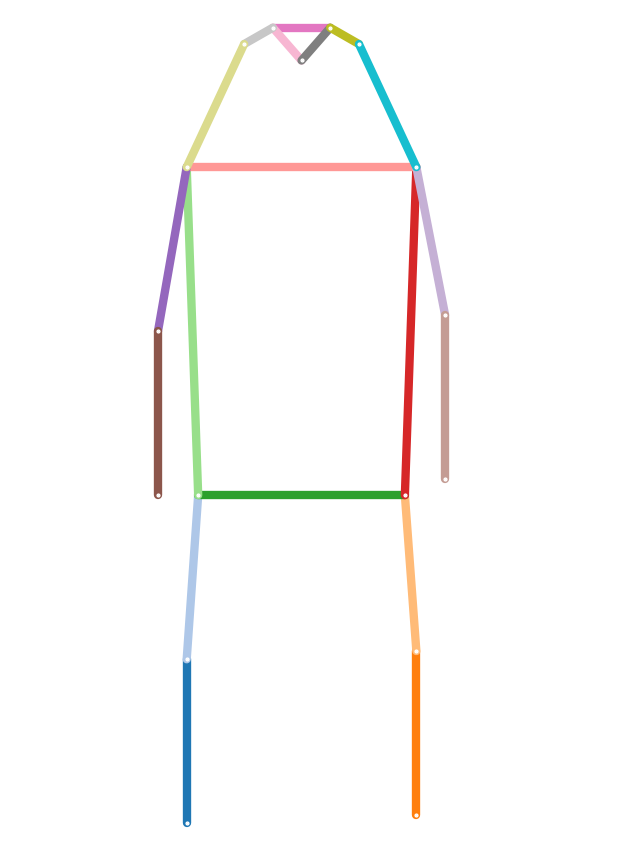
\includegraphics[width=.3\textwidth]{./images/coco_topology.png}
	\caption{Топология COCO}
	\label{fig:coco_topology}
\end{figure}

\subsubsection*{Подходы к распознаванию}

Другим вопросом для описываемой задачи стал подход к распознаванию. Делать детекцию человека и уже на кропнутом изображении производить поиск или искать все возможные точки, а потом собирать их в скелет. Эти две идеи и сформировали два направления развития методов HPE. Немного о них:
\begin{enumerate}
	\item \textit{Подход сверху-вниз (англ, top-down)}\\
	Для данного этапа вам понадобится дополнительная модель детекции, которая локализует человека на изображении, выделяя его в прямоугольную область. Затем этот прямоугольник передается в модель распознавания ключевых точек. Этот подход обеспечивает высокую точность предсказания КТ, но может быть чувствителен к ошибкам на этапе обнаружения и ориентации человека в кадре, что требует дополнительной предобработки изображений.
	\item \textit{Подход снизу-вверх (англ, bottom-up)}\\
	Для данного подхода вам не нужны помощники в виде детектора, но все равно имеет два этапа в своей работе. Первоначально модель распознает все ключевые точки на полученном на вход изображении, получая таким образом карту распределения КТ по фото. А вторым шагом модель собирает все полученные точки единый скелет. При детекции нескольких людей необходимо верно сопоставить их части тела. Для этого есть несколько способом, один из которых является построение полей сходства частей тела (part affinity fields), используемый в проекте OpenPose \cite{OpenPose}.
\end{enumerate}

Несмотря на различия в описанных подходах, результатом их работы является массив данных размера $[N \times K \times 3]$, где $N$ - количество распознанных человек, $K$ - количество ключевых точек в топологии, а 3 представляет два номера пикселей на изображении и координату видимости точки. Последнее часто интерпретируется как уверенность модели в обнаруженной точке.

\newpage %% Распознавание ключевых точек
    \section{Доменная адаптация}
\label{sec:Chapter3} \index{Chapter3}

В современном мире машинного обучения и искусственного интеллекта способность моделей адаптироваться к новым условиям и данным стала одной из ключевых задач. Традиционные методы обучения моделей предполагают, что данные, используемые для обучения и тестирования, имеют схожие характеристики и распределения. Однако в реальных приложениях часто возникает необходимость применять модели на данных, которые существенно отличаются от тех, на которых они были изначально обучены. Это приводит к снижению точности и эффективности моделей, что ставит под угрозу их практическое применение.

Для решения данной проблемы была разработана задача доменной адаптации, целью которой является создание методов для акклиматизации модели к целевым данным, отличающимся от исходных. В рамках этой задачи были разработаны подходы и техники, направленные на уменьшение расхождений между исходным и целевым доменами, что позволяет сохранять точность и производительность моделей в новых условиях. Эти методы способствуют переносу знаний, накопленных в исходном домене, на целевой, что относит данную задачу к области методов transfer learning.

\subsection{Перенос знаний}

Перенос обучения (англ. transfer learning) позволил уже существующим решениям выйти за пределы первоначально заданных задач. Этот подход позволил использовать различные архитектуры для решения новых, разнообразных проблем. К примеру, это позволило перенести опыт использования трансформеров из задач обработки естественного языка в задачи компьютерного зрения.

Помимо переноса знаний между различными областями нейронных сетей, transfer learning предоставляет возможность использовать опыт, накопленный в процессе обучения модели, для работы с новыми данными. Эти данные могут представлять собой не только новые классы в задачах классификации или кластеризации, но и иметь значительные структурные различия, такие как язык и жанр для текстовых данных или стиль и качество для изображений. Такие методы, называемые адаптацией к новым доменам данных, позволяют существенно сократить время и ресурсы, направленные на решение новых, узкоспециализированных задач.

\begin{figure}[h]
	\centering
	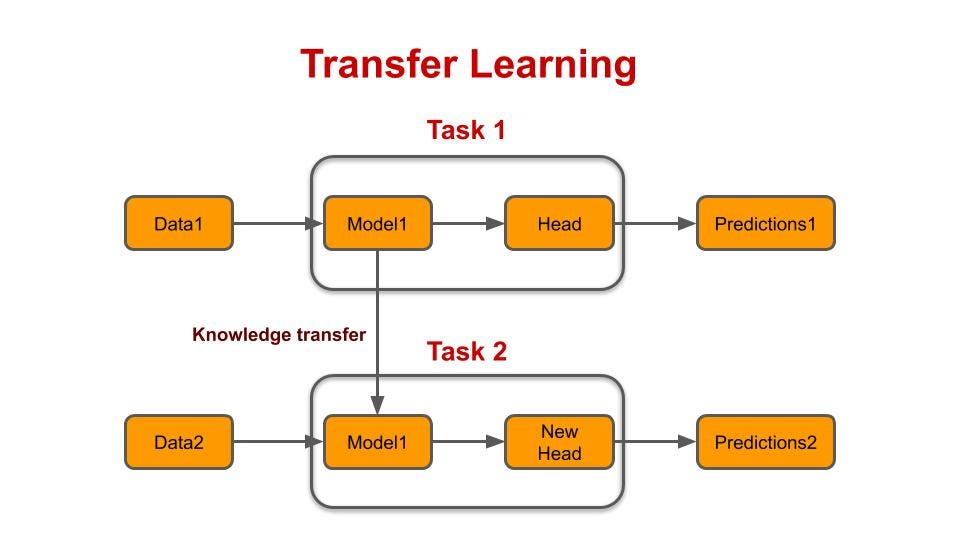
\includegraphics[width=\textwidth]{./images/TL_medium.jpg}
	\caption{Основная идея переноса знаний}
	\label{fig:tl}
\end{figure}

Основная идея состоит в том, чтобы взять модель, которая уже научилась извлекать и интерпретировать общие признаки из большого набора данных, может эффективно адаптироваться к новым данным, требующим более специфических знаний (см \autoref{fig:tl}). Это аналогично тому, как человек, обладая общими знаниями в одной области, может быстрее освоить смежную сферу деятельности. Таким образом получается не только ускорить процесс обучения, но и повысить точность и эффективность модели при условии ограниченности в ресурсах. 

\subsection{Основные определения}

Для дальнейшего повествования введем формальные обозначения для данной задачи.

\underline{Определение домена}

Пусть существует пространство признаков $\chi$ и в нем задан набор данных $X$ и частотное распределение вероятностей на нем $P(X)$:
\begin{equation}
	X = {X_1, ..., X_n} \in \chi.
\end{equation}

В таком случае \textit{доменом $D$} называют совокупность пространства признаков и частотного распределения вероятности на заданном наборе данных:
\begin{equation}
D = \{\chi, P(X)\}
\end{equation}

\underline{Определение задачи}

Пусть на пространстве признаков $\chi$ задан набор данных
\begin{equation}
	X = \{X_1, ..., X_n\} \in \chi.
\end{equation}

Пусть существует пространство меток $\gamma$ и для заданного набора данных существует соответствующий набор меток
\begin{equation}
Y = \{Y_1, ..., Y_n\} \in \gamma
\end{equation}

Тогда \textit{задача $T$} определяется как 
\begin{equation}
T = \{Y, f(X)\},
\end{equation}
где $f$ - прогностическая функция зависимости целевой переменной, которую можно рассматривать как условное вероятностное распределение $P(Y|X)$.\\

\underline{Определение доменной адаптации}

В задаче доменной адаптации подразумевается наличие не менее двух наборов данных:
\begin{enumerate}
\item \textit{Исходный домен (Source)}\\
Представляет собой универсальный набор данных большого объема. Обозначается следующим образом:
$$D^s = \{\chi^s, P(X^s)\}$$
На домене определена задача: $$T^s = \{Y^s, f^s(X^s)\}$$
\item \textit{Целевой домен (Target)}\\
Представляет собой набор данных маленького объема, к которому планируется адаптировать модель. Обозначается следующим образом:
$$D^t = \{\chi^t, P(X^t)\}$$
На домене определена задача: $$T^t = \{Y^t, f^t(X^t)\}$$
\end{enumerate}

В зависимости от того, как соотносятся между собой домены $D^S$ и $D^T$ и задачи $T^s$ и $T^t$, ставятся различные задачи:
\begin{enumerate}
\item Самым распространенным является случай совпадения задач и доменов, когда $D^s = D^t$ и $T^s = T^t$. В таком случае говорят о постановке задачи классического машинного обучения. Домен $D^s$ называют обучающей выборкой, которая используется для обучения решения $T$, а домен $D^t$ - тестовой выборкой, на которой производится оценка правильности полученного решения.

\item При совпадении данных $D^S = D^t$, но различной постановке задачи $T^s \ne T^t$ говорят о мультизадачном обучении. Часто такая постановка задачи подходит для адаптации модели классификации к новым меткам классов, которые представлены в целевой выборке, но отсутствуют в исходной.

\item При совпадении задач $T^s = T^t$, но различии в данных $D^s \ne D^t$ говорят о методах кросс-доменной адаптации. В таком случае ставится задача улучшения предсказания $T^t$ с использованием информации, полученной в $T^s$. 

\item При полном несовпадении данных $D^S \ne D^t$ и задач $T^s \ne T^t$ подразумевается, что пары $(D, T)$ решают разные проблемы и адаптация происходит в индивидуальном порядке. Например, использование архитектуры трансформер, зарекомендовавшей себя в задачах обработки естественного языка, для задач компьютерного зрения.
\end{enumerate} 

\begin{figure}[h]
	\centering
	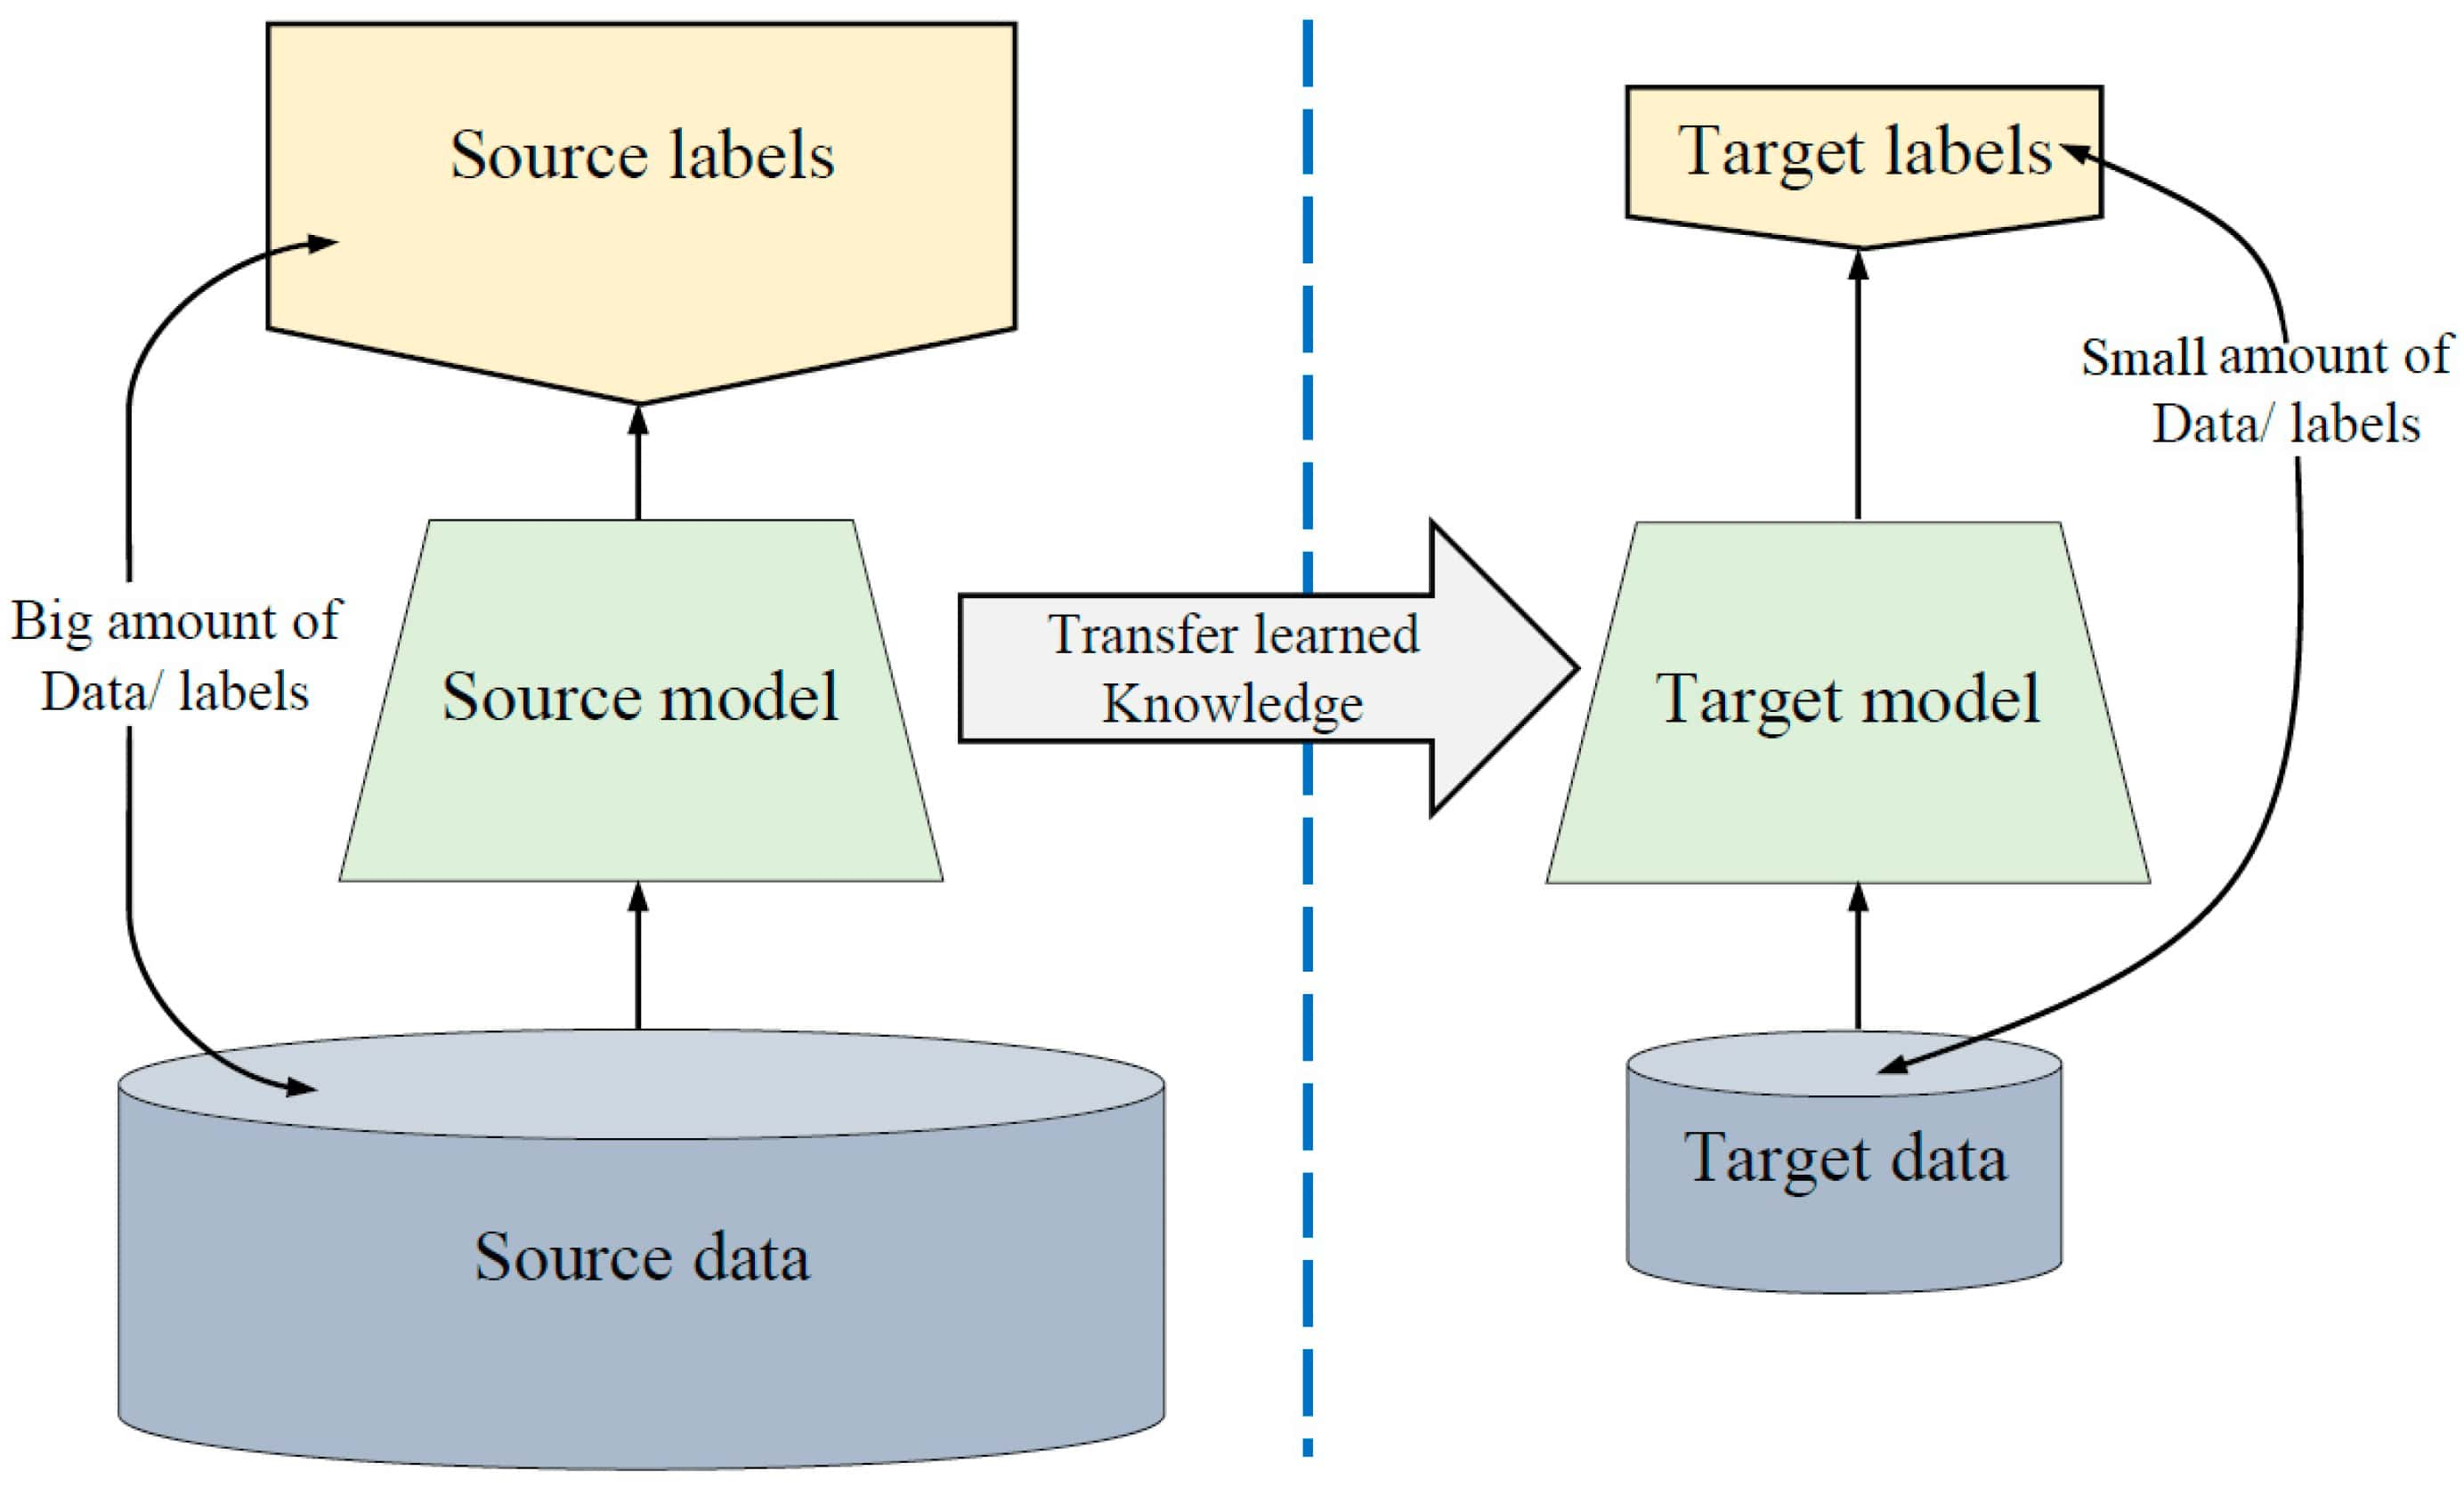
\includegraphics[width=.75\textwidth]{./images/DA.jpg}
	\caption{Схематическое представление работы алгоритмов доменной адаптации}
	\label{fig:DA}
\end{figure}

В текущей работе рассматривается третий вариант: $D^s \ne D^t$, но $T^s = T^t$. Схематически постановка задачи описана на \autoref{fig:DA}, а формулировка задачи математическим языком выглядит следующим образом:
$$D^s, T^s \to D^t, T^t$$

\subsection{Классификация методов доменной адаптации}

Ранее методы, которые решают задачу \textit{доменной адаптации (англ. domain adaptation)}  были определены как методы переноса знаний, направленные на на приспособление моделей $T^s = T^t = T$, обученных на данных из домена $D^s$, к данным из домена $D^t$, причем $D^s \ne D^t$. Данные могут различаться по различным характеристикам и в зависимости от различают несколько типов методов, которые схематически представлены на \autoref{fig:DA_classification}.

\begin{figure}[h]
	\centering
	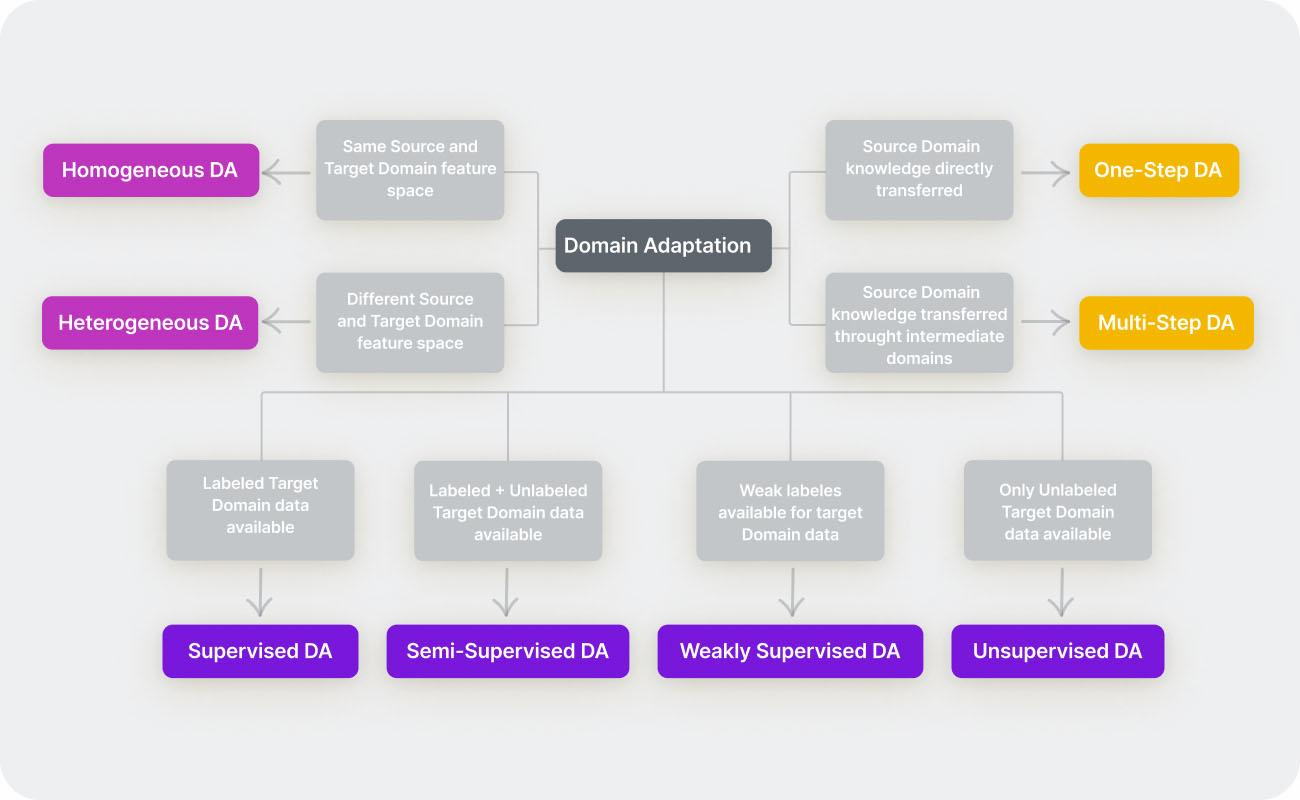
\includegraphics[width=.85\textwidth]{./images/DA_classification.jpg}
	\caption{Схематическое представление работы алгоритмов доменной адаптации}
	\label{fig:DA_classification}
\end{figure}

В зависимости от того, насколько сопоставляются распределения наборов данных $P(X)$ различают гомогенные и гетерогенные методы:

\begin{enumerate}
\item \textit{Гомогенные методы (Homogeneous DA)}

Данный тип методов применяется, когда исходный и целевой домены имеют одинаковое пространство признаков $\chi^s = \chi^t = \chi$, но их распределения отличаются $P(X^s) \ne P(X^t)$. Методы гомогенной адаптации фокусируются на выравнивании распределений признаков между доменами, чтобы модель, обученная на исходных данных $D^s$ , могла эффективно работать на целевых данных $D^t$.

\item \textit{Гетерогенные методы (Heterogeneous DA)}

В отличие от предыдущих способов, в текущем случае отличаются и признаковые пространства между доменами $\chi^s \ne \chi^t$. Это представляет собой более сложный сценарий, так как необходимо либо преобразовывать целевые данные в такое представление, которое будет сопоставимо с исходными, либо выуживать обобщенные признаки из обоих доменов, на которых модель будет считать данные похожими.

\end{enumerate}

\hfill \break
Также стоит обратить внимание насколько сильно отличаются распределения данных, так как от этого зависит сколько шагов необходимо будет производить между доменами:

\begin{enumerate}
\item \textit{Одношаговая доменная адаптация (One-step DA)}

При небольших различиях между распределениями можно использовать прямой перенос знаний из $D^s$ в $D^t$. В таком случае опыт, накопленный моделью в исходном домене, напрямую используется при адаптации модели $T$ на целевом домене. Преимущества этого метода заключаются в его простоте и быстроте внедрения, так как он не требует промежуточных шагов.

\item \textit{Многошаговая доменная адаптация (Multi-step DA)}

Однако эффективность One-Step DA может снижаться, когда различия между исходным и целевым доменами слишком велики для прямого переноса знаний. Для этих случаев и используются методы многошаговой адаптации. Они подразумевают поэтапное выполнение: знания из исходного домена сначала переносятся в один или несколько промежуточных доменов, прежде чем достигнуть целевого. Промежуточные шаги помогают постепенному выравниванию распределения данных, что улучшает адаптацию и повышает точность модели в целевом домене.

\end{enumerate}

\hfill \break
Последним маркером в классификации методов доменной адаптации является доступность размеченных данных для $D^t$. По данному признаку методы разделяются сразу на 4 группы:

\begin{enumerate}
\item \textit{Supervised domain adaptation}

В этом случае обучение модели происходит с использованием как исходных, так и целевых данных, имеющих метки. Поэтому данные методы обычно достигают высокой точности, поскольку модель может явно учиться на целевых данных с метками.

\item \textit{Semi-supervised domain adaptation}

К данным методам прибегают, когда в целевом домене присутствуют как размеченные данные, которые используются для начального обучения, так и неразмеченные данные, на которых есть возможность улучшать работу модели. 

\item \textit{Weakly supervised domain adaptation}

Когда данные целевого домена слабо размечены, то есть использовалась автоматическая система разметки, которая допускает ошибки, используются методы weakly supervised DA. Они направлены либо на улучшение точности слабых меток, либо используют <<мягкие>> техники регуляризации, что позволяет учитывать возможность ошибки в данных.


\item \textit{Unsupervised domain adaptation}

Самый сложный случай, когда нет возможности аннотировать домен и надо на сырых данных улучшить качество модели. Для методов этого типа часто используется кластеризация данных и итеративные подходы, которые помогают модели $T$ улучшать собственные предсказания.

\end{enumerate}


\newpage %% Доменная адаптация
    \section{Обзор существующих решений}
\label{sec:Chapter4} \index{Chapter4}

В данной главе необходимо провести анализ существующих моделей. Аргументировать выбор тех или иных моделей, методов. Подготовить теоретическую базу перед экспериментов.

\subsection{Обзор моделей для распознавания КТ}

\subsubsection{DeepPose}

Чисто для исторической справки. Если нужен будет объем.

\subsubsection{AlphaPose}

Чисто для исторической справки. Если нужен будет объем.

\subsubsection{OpenPose}

??? год. Проект от лаборатории ??? от института ???. 

Показала хорошие результаты при предыдущих сравнениях. Использует

\subsubsection{BlazePose}

Проект MediaPipe от гугл использует сеть архитектуры BazePose.

Показывает хорошие результаты. Имеет хорошие

\subsubsection{HRNet}

2019 год. Основная модель от проекта MMPose. Использует интересную архитектуру и хорошо показала себя при предыдущих сравнениях.

\subsubsection{ViTPose}

Трансформер. ??? год. Интересная архитектура. Рассказать про трансформер, рассказать про кодеки/докедеки. Рассказать про способ работы. Можно расписатьсся неплохо.

\subsubsection{RTMPose}

2023 год. На момент ислледования наиболее актуальная модель от проекта MMPose.

Работает неплохо. Обучается тоже неплохо. Попробуем заюзать в экспериментах.

\hfill \break

ОБЗОР ДАЛЬНЕЙШИХ РЕШЕНИЙ ПОЗЫ ПОД БОЛЬШИМ ВОПРОСОМ.

\subsubsection{Swin}

Трансформер. 2021 год. Все )

\subsubsection{Simcc + Resnet}

Вообще хз что это, но если смогу, то сделаю эксперимент )

\subsubsection{Dekr + HRNet}

Подход снизу вверх. ??? год. Модель, обученная лабораторией показывает хорошие результаты, но очень прожорлива в плане ресурсов для обучения.

\subsubsection{YoloPose}

Несколько различных версий архитектуры Yolo дают несколько различных версий модели для распознавания позы. Использует подход снизу-вверх и хорошо


\subsection{Анализ и выбор методов доменной адаптации}

Опираясь на модели из предыдущей главы надо сделать анализ и выбрать только несколько методов, которые применимы к нашим требованиям и которые мы будем сравнивать между собой.

\subsubsection{PUL}

Будем это использовать в работе. Надо будет хорошо расписать...

\subsubsection{RegDA}

Интересный алгоритм. На нем базируются все остальные

\hfill \break

ПРИ НЕХВАТКЕ ВРЕМЕНИ МОЖНО БУДЕТ ОСТАВИТЬ ТОЛЬКО ОДИН ИЗ СЛЕДУЮЩИХ МЕТОДОВ.

\subsubsection{UDA PoseEstimation}

Адаптация от синтетических данных к реальным. Должно бтыь интересно описать. Не использовали, так как до сих пор мы не перешли в 3х мерное пространство.

\subsubsection{POST}

Похожее на предыдущее

\subsubsection{SFDA}

Похожее на предыдущее


\newpage
 %% Обзор существующих решений
    \section{Эксперимент}
\label{sec:Chapter5} \index{Chapter5}

В данной главе будет описан эксперимент, как таковой.

\subsection{Описание деталей эксперимента}

Постановка эксперимента. Что планируется сделать и какие результаты хочется получить. Какие метрики будем использовать и по каким метрикам будем сравнивать.

\subsection{Данные. Сбор и разметка}

Описание собранных данных. Численный объем датасета. Возможно количество локаций и распределение по ним.

Необходимо предоставить данные по распределению данных между людьми, по количеству данных для обучения/тестирования. Предоставить данные по локациям. Предоставить картинки с примерами данных, которые были собраны.

Описание системы полуавтоматической разметки данных. Что там использовалось и как проходит разметка.

Для разметки собранных данных была создана система полуавтоматической разметки данных pose-markup (ССЫЛКА). Система состоит из двух частей: автоматическая разметка ключевых точек с помощью нейросети от MediaPipe и корректировка полученных данных экспертом.

На данный момент проект ориентирован на разметку позы только на видео файлах, так как это было необходимо реализовать в рамках эксперимента. В будущем планируется добавить возможность размечать точки и на одиночных изображениях.

Добавить коллаж примера рботы системы (3 фото: исходное, после автоматической разметки, после корректировки. Необходимо явно указать точки, которые были изменены.)

Численные данные о разметке данных. Сколько пришлось разметить, сколько пришлось скореектировать. Предоставить некоторые картинки по распределению корретировки данных.

В рамках разметки данных можель имела неточности, поэтому роль эксперта была существенна при валидации работы автоматической части системы. Процент фотографий на которых были проведены изменения: собрать статистику и предоставить результаты корректировки разметки: сколько суммарно точек было изменено, сколько точек имели изменения более 5\% от роста человека (метрика в бакалаврском дипломе есть), тоже самое для 15\%, три случая для среднего количества точек на фотографии, три случая для фотографий (может большинство изменений были на трети фотографий, а остальные не меняли), представить сводную таблицу изменений для точек по топографии КОКО, визуализировать сводную таблицу на картинке. 

\subsection{Результаты эксперимента}

Предоставить относительно сухо результаты эксперимента. Можно дать базовый анализ ситуации и того, что мы видим.

Необходимо предоставить результаты по времени обучения нейросетей, времени дообучения нейросетей. \\ 
Собрать данные по количеству ошибок до-после обучения. Собрать данные по количеству ошибок при изменении домена. \\ 
Данные по ресурсам, на которых обучались нейросетки.


\newpage %% Эксперимент
    \section{Заключение}
\label{sec:Chapter6} \index{Chapter6}

%Необходимо рассказать о результатах исследования и о том, что мы получили. Привести сравнения, если таковые будут иметь место. Закинуть удочку для будущих исследований.

В рамках проведенного исследования были рассмотрены несколько решений задачи распознавания ключевых точек на теле человека, а также некоторые способы доменной адаптации без учителя. В качестве практической части работы была оценена применимость метода адаптации progressive unsupervised learning, основанного на генерации и фильтрации псевдо-размеченных данных, к моделям оценки позы. 

Для эксперимента был собран и частично аннотирован набор данных для оценки позы боксеров во время тренировки. Чтобы упростить автоматизацию процесса разметки была создана полуавтоматическая система pose-markup с использованием нейросетей, не задействованных в рамках исследования.

В результате имеются следующие выводы:

\begin{itemize}
\item При использовании в качестве функции фильтрации отсеивание поз по средней уверенности точек в ней, необходимо выбирать порог доверия не менее 0.5. Иначе в выборку будет попадать большой объем ошибочных данных, в которых модель не очень уверена, и результаты адаптации будут монотонно ухудшаться;
\item Наилучший результат адаптации был получен при использовании алгоритма SimCC  с магистральной нейронной сетью ResNet. В рамках доменной адаптации было повышено количество верно распознанных ключевых точек для метрики PCK с пороговым значением 0.5 и улучшена точность уже имеющихся предсказаний;
\item Отсутствие необходимости в разметке целевых данных экономит множество ресурсов, ведь генерация псевдо-разметок на домене объемом примерно 2200 изображений занимала не более 10 минут на итерацию, а аннотирование этих данных с помощью pose-markup заняло не менее 74 часов;
\item При наличии сложно различимых частей тела на изображениях стоит выбирать другую функцию фильтрации, так как предсказания этих ключевых точек будут сильно ухудшать возможности адаптации.
\end{itemize}

Дальнейшие планы развития данной темы включают в себя поиск новых методов фильтрации псевдо-разметок, основанных на анализе тепловых карт и их производных, сравнение результатов работы полученного метода с другими способами адаптации моделей к целевым доменам, расширение полученного набора данных новыми локациями и людьми.

\newpage %% Заключение
          
    
    %% Don't change the following lines
    \nocite{*}
    \phantomsection
   	\addcontentsline{toc}{section}{Список литературы}
    \bibliography{references}

    %% в зависимости от надобности подключаем раздел "Приложениие"
    % \newpage
    % \section{Приложение}
\label{sec:Apendix} \index{Apendix}

Здесь необходимо написать приложение, которое вы должны придумать самостоятельно
\end{document}